\chapter{Background}\label{chap:background}
This chapter briefly introduces the theoretical and practical components
involved in design and implementation of the Dual programming language and its
environment. 

\section{Web technologies}
As stated in the introduction, one of the main design goals of the system is usability. This is accomplished in practice by building on top of the most accessible and ubiquitous platform -- the web platform\cite{web_platform}\footnote{Also referred to as the \textit{open} web platform\cite{open_web_platform}}.

The language's interpreter and development environment are intended to work with
and are built on web technologies: JavaScript, HTML5 and CSS. The prototype
implementation makes use of Node.js, a server-side JavaScript runtime\cite{nodejs_site} and
CodeMirror, a JavaScript library which provides basic facilities for the text-based code editor part of the system\cite{codemirror_site}. This part is modeled after modern web-oriented code editors with similar design philosophy\cite{js_text_editors_wikipedia}, such as Visual Studio Code\cite{vscode_site}, Brackets\cite{brackets_site}, Atom\cite{atom_site} and many others.

\subsection{Document Object Model}
The \acrlong{dom} (\acrshort{dom}) is an interface that lets JavaScript manipulate HTML documents as tree structures. The interface aims to be independent of a platform or programming language and is not limited to JavaScript and HTML\cite{dom_spec, w3_dom, dom_wikipedia}. 

In the DOM, each part of the document is represented by a node in a tree manipulable by JavaScript. All changes applied to the tree can be reflected in the document immediately and displayed.

The DOM structure can be manipulated with JavaScript in the following ways\cite{w3s_dom}:
\begin{itemize}
\item All of the document's elements and their attributes can be changed or removed.
\item New elements and attributes can be added.
\item The whole tree structure can be easily traversed, as each node contains references to many other nodes: its parents, children (with separate references to the first and last child) or siblings.
\item All the CSS styles assigned to the document and individual elements can be changed. This means manipulating the details of how the elements are laid out and displayed. An enormous number of different display properties can be customized\cite{mdn_css_ref}, such as colors, fonts, sizes, etc.
\item JavaScript can react to all existing HTML events, such as clicking on elements, scrolling the page that contains the document, etc.
\item JavaScript can create new events.
\end{itemize}

\subsection{JavaScript}
The JavaScript programming language was created by Brendan Eich for Netscape\cite[Introduction]{ecmascript}, the company which created the Netscape Navigator web browser. There is a line of evolution that leads from Netscape and its browser to Mozilla and Firefox\cite{netscape_mozilla, mozilla_story}. The language was developed in 10 days in April 1995\cite{js_ten_days}.

Despite significant design flaws, JavaScript has became \textit{one of} the most\cite{tiobe, pypl}, if not \textit{the most}\cite[Section~Most Popular Technologies per Dev Type]{so_developer_survey_2016}\cite{redmonk} popular programming languages in the world. In this section I will briefly look at some of the probable reasons for that from a programming language design perspective.

From a programming language design perspective, JavaScript has many great
features, borrowed from excellent languages\cite[Section~4~Overview]{ecmascript}, most notably:
\begin{itemize}
   \item Scheme, one of two main dialects of Lisp\cite{r7rs}. It is a minimalist, but very extensible functional programming language. The features drawn from this language include first-class functions (treating functions as values), anonymous functions (also known as lambdas or function literals) and lexical closures.
   \item Self, a pioneering prototype-based \acrlong{oop} language\cite{self_handbook}, which evolved from Smalltalk-80\cite{smalltalk_history}. It introduced the concept of prototypes, which is an approach to \acrshort{oop}, where inheritance is implemented by reusing existing objects instead of defining classes. Prototype-based programming is the feature that JavaScript adopted from this language.
\end{itemize}

The two above languages are characterized by a very minimalist nature.
Both languages as well as JavaScript\cite{js_types} are dynamically typed -- types can be checked only at runtime. 

The final advantage of JavaScript is the fact that it is distributed with a ubiquitous environment of the web browser. This makes the language straightforward for developers to use.
Easy to get started -- attract novice developers
Reach billions of users\cite{internet_stats}

The above mixture turns out to create a very powerful and usable language.


In the recent years JavaScript's popularity has been steadily growing\cite{js_growth}. This translated to significant improvements in the language's standarization efforts. Since 2015, ECMA International's\cite{ecma} Technical Commitee 39\cite{tc39}, the commitee which defines ECMAScript -- the official standard for JavaScript -- adopted a new process. Under this process, a new version of the standard is released annually\cite{ecmascript, ecmascript_2015, ecmascript_2017}. The documents and proposals are publicly available at GitHub\cite{ecma_github}.


Static type checking for JavaScript is also possible with Flow\cite{js_flow} -- a static type checker, which works either as a syntax extension or through comment annotations -- or TypeScript\cite{typescript} -- which is a superset of JavaScript.

\subsubsection{Concurrency model}
In the context of the concurrency model, the JavaScript runtime conceptually
consists of three parts: the call stack, the heap and the message queue. All
these are bound together by the event loop\cite{mdn_concurrency}, which is the crucial part of this model.  An iteration of this loop involves the following steps:
\begin{enumerate}
	\item Take the next message from the queue or wait for one to arrive. At
          this point the call stack is empty.
	\item Start processing the message by calling a function associated with
          it. Every message has an associated function. This initializes the
          call stack.
	\item Processing stops when the stack becomes empty again, thus
          completing the iteration.
\end{enumerate}

This means, at least conceptually, that messages are processed one by one, in a single thread and an executing function cannot be preempted by any other function before it completes. In practice this is more complicated and there are exceptions to these rules. But this explanation is sufficient for further discussion.

This model makes reasoning about the program execution very straightforward, but
is problematic when a single message takes long to execute. The problem is
observed e.g. when web applications cause browsers to hang or display a
dialog asking the user if she wishes to terminate an unresponsive script.

For this reason it is best to write programs in JavaScript that block the event
loop for as short as possible and divide the processing into multiple messages.

This concurrency model is called the \textit{event} loop, because the messages are added to the queue any time an event occurs (an has an associated handler), such as a click or a scroll. In general input and output in JavaScript is performed asynchronously, through events, so it does not block program execution.

\section{Design and implementation of Lisp}\label{sec:lisp}
A very important family of programming languages and one which had the most
influence on the design of Dual is the Lisp family. In this thesis I use the
singular form ``Lisp'' to refer to the whole family rather that a concrete
dialect or implementation -- such as Common Lisp\cite{common_lisp_hyperspec}, Scheme\cite{r7rs}, SBCL\cite{sbcl_site} or Racket\cite{racket_site} -- unless otherwise noted.

Lisp is characterized by a very minimal syntax, which relies on Polish (prefix)
notation for expressions and parentheses to indicate nesting. There are only
expressions and no statements in the language. This means that every language
construct represents a value. There is also no notion of operator precedence.

The two core components of a Lisp interpreter are the \texttt{apply} and
\texttt{eval} functions\cite[Section~4.1]{sicp, c2_eval_apply}. The
former takes as arguments another function and a list of arguments and applies
this function to these arguments. The latter takes as arguments an
\texttt{expression} and an \texttt{environment} and evaluates this expression in
this environment. The typical implementation of \texttt{eval} distinguishes
between a few types of expressions. The essential are:
\begin{itemize}
	\item Symbols (also known as identifiers or names) --
          e.g. \texttt{velocity} -- these are evaluated by looking up the value
          corresponding to the symbol in the environment, so \texttt{velocity}
          might evaluate to \texttt{10} if it is defined as such in the
          \texttt{environment}
	\item Numbers (or number literals) -- e.g. \texttt{3.2} -- these
          evaluate to a corresponding numerical value
	\item Booleans (boolean literals) -- \texttt{true} or \texttt{false} --
          evaluate to a corresponding boolean value
	\item Strings (string literals) -- e.g. \texttt{"Hello, world!"} --
          evaluate to a corresponding string value
	\item Quoted expressions -- e.g. \texttt{'(+ 2 2)} -- a quoted
          expression evaluates to itself; in other words a quote prevents an
          expression from being evaluated
	\item \textit{Special forms} or \textit{primitives}, which are
          expressions that have some special meaning in the language. These are
          the basic building blocks of programs. For example:
	\begin{itemize}
		\item \texttt{if}, the basic conditional expression and other
                  flow control expressions; the special meaning of these is that
                  they evaluate their arguments depending on some condition
		\item \textit{lambda} expressions -- essentially function
                  literals, which consist of argument names and a body
		\item \textit{definition} and \textit{assignment} expressions;
                  these modify the environment; usually they treat their first
                  argument as a name of the symbol in the environment, so it is
                  not evaluated; the second argument is evaluated and its value
                  is associated with the symbol
	\end{itemize}
\end{itemize}

A Lisp expression can look like this:
\begin{lstlisting}[label={lst:lisp_expression}]
(+ 2 (* 3 5))
\end{lstlisting}

Words are delimited by white space. Each sequence of words between parentheses can be viewed as a list\footnote{Originally the name Lisp was an acronym, which stood for ``LISt Processing''\cite[Section~1.2]{emacs_lisp_reference}\cite[Chapter~12]{practical_lisp}}. Lists can be nested inside each other. Each list represents an expression, where the first element of the list is the expression's operator and the following elements are its arguments.

This parenthesized notation is called S-expressions\cite[Section~Recursive Functions of Symbolic Expressions; Section~The LISP Programming System]{s_expressions}. These are used to represent both code and data. For example the code from Listing \ref{lst:lisp_expression} can be represented (in Common Lisp\footnote{All the remaining listings in this section contain code in Common Lisp.}) as data:
\begin{lstlisting}
(list '+ 2 (list '* 3 5))

; or shorter equivalent:
'(+ 2 (* 3 5))
\end{lstlisting}

Where \texttt{list} is a function that produces a list that contains the values of its arguments.

\texttt{'} is a \textit{quote} symbol. It prevents an expression from being evaluated.

\texttt{;} begins a comment that extends to the end of current line.

\texttt{+} and \texttt{*} are functions that perform their corresponding arithmetic operations: addition and multiplication respectively.

This data representation can now be manipulated. For example:
\begin{lstlisting}
; set the `expression` variable to hold the same list value
; as in the above listing:
(setf expression '(+ 2 (* 3 5)))

; the variable `expression` now represents
; the expression `(+ 2 (* 3 5))`

; replace `*` with `exp` in the `expression`
; since it is just an ordinary list,
; this is done with ordinary data manipulation functions:
(setf (first (third expression)) 'expt)

; the variable `expression` now represents
; the expression `(+ 2 (expt 3 5))`
\end{lstlisting}

Where \texttt{setf} evaluates its second argument and stores it in a variable represented by its first argument. The first argument can be -- among other things\cite[Section~11.15.1]{emacs_lisp_reference} -- the name of the new variable or a place in an existing list. 

\texttt{first} and \texttt{third} take a list as an argument and extract the first or the third element from that list accordingly.

\texttt{expt} is a function that performs exponentiation: it takes two numerical arguments and returns the value of the first raised to the power determined by the value of the second.

We can now evaluate the \texttt{expression}:
\begin{lstlisting}
; returns 245, which is the result of
; evaluating (+ 2 (expt 3 5)):
(eval expression)
\end{lstlisting}

\texttt{eval} here is a function of one argument -- an expression to be evaluated in the current environment. This is ``a user interface to the evaluator''\cite[Section~3.8, Function~EVAL]{common_lisp_hyperspec} (which can be understood as the internal function \texttt{eval} described at the beginning of this section).

The property of representing code and data in essentially the same form is known as homoiconicity\cite{homoiconicity_wikipedia, c2_homoiconicity, homoiconicity}. In the case of Lisp an S-expression can be very straightforwardly mapped to a corresponding \acrlong{ast} (\acrshort{ast}) node.

%For detailed explanation please refer to \cite{sicp}.

\subsection{Abstract syntax tree and program representation}
The term \acrshort{ast} refers to a tree data structure that is built
by parsers of programming languages to represent syntactic structure of source
code in an abstract as well as easily traversable and manipulable way. In the simplest form, in expression-only languages such as Lisp each node of such tree
represents a single expression. The tree is abstract in the sense that it does
not necessarily contain all the syntax constructs that occur in the source code
or encodes them in some \textit{abstract} way. In case of Lisp, there's no need to store or represent bracketing characters \texttt{()} in the AST, as nesting is inherent in the data structure itself.

In theory, a programming language does not require a text representation and
could be defined only in terms of a data structure such as a syntax
tree. Practically, for a language to be useful, it needs to come with an
editable representation that provides a convenient way for a programmer to
construct programs. Currently the most successful representation for that is the
human-readable text-based representation, which evolved from more primitive and
less convenient representations, such as punched cards\cite{columbia_history_cards, punched_cards_wikipedia}.

\subsection{Text-based code editors}\label{sub:text_editors}
Constructing programs with text representation can be done with any text editor. This means that the representation is largely independent of a tool, which is an advantage. Any application capable of editing text can theoretically be used to edit any source code (ignoring details such as encoding, etc.). Such applications are universally available, so source code stored in text files can be edited freely on any platform with any tool.

But for complex programs a simple text editor quickly becomes inconvenient and a
more specialized one is preferable. Such code editors introduce various features
that greatly improve the convenience of working with a text-based representation
of a programming language. For example:
\begin{itemize}
	\item Automatic structuring of the text to emphasize blocks of code
          (auto-indentation).
	\item Highlighting of different syntactic constructs with different colors.
	\item Context-based auto-completion.
	\item Automatic correction of errors.
	\item The ability to fold distinct blocks of code.
	\item Advanced navigation through the code: jumping to declarations,
          definitions, other modules or files.
\end{itemize}

Most of these features require that the editor makes use of a parser to
recognize the syntactic structure of a program.

Other advantages of a text representation, that stem from the multitude of ways
that raw text can be manipulated and processed and are not related to any particular syntax:
\begin{itemize}
	\item Find and replace with regular expressions.
	\item Selecting/processing many lines or even blocks of text.
	\item Editors often treat the source as a 2D grid of characters; each
          row and column of such grid can be numbered.
	\item Debuggers, compilers and other elements of a programming language
          system can use row and column numbers in error messages.
	\item Version control systems can easily compare (diff) and keep track of changes in text files.
\end{itemize}

\subsection{Visual programming languages}\label{sec:vpls}
An alternative representation is the one employed by visual programming
languages. By a visual programming language I mean a language that ``lets users create programs by manipulating program elements graphically rather than by specifying them textually''\cite{vpl_wikipedia, vpl_maturity}.

Such languages are usually tied to a particular editor, which allows
the programmer to edit the source code with a mouse rather than the
keyboard. That is instead of typing in streams of characters to be parsed and
assembled into a structural form, the programmer inserts, arranges and connects together distinct visual elements to produce such a structure. Thus I contend that visual programming can be defined at the lowest level as manipulating a visual form of a language's syntax tree.

The design of the visual representation for my language involved a rough survey
of visual programming languages. In this section I will describe the results obtained from this survey.

I classified each of nearly 160 languages listed in \cite{snapshots}, according
to type of their visual representation into several categories.

Additionally, I associated each language with a number $s \in [0, 3]$, which
descirbes its ``structure factor''. This quantifies my subjective assessment of the readability of the representation compared to familiar text representation ($s = 3$). For example, if it appears that the representation consists of scattered blocks, connected by lines and the layout seems to be arranged by the user, with no editor-support for automatic structuring, $s$ will be low. In other words, the greater the number, the better structured the representation.

This analysis is not strict and systematic, but rather heuristic-based. A language is classified based solely on the screen shots from its environment. Its purpose is to assess general trends and determine which solutions gained the greatest adoption in practice. This is to aid the further design process. 

Below I present the results of this classification in the form of a list. The items are organized as follows:

\begin{itemize}
    \item <<Name of category>> -- <<percentage of languages that fall into the
category>> -- <<the average ``structure factor'' $s$ for the category>>

    <<short description>>
\end{itemize}

Here are the compiled results:
\begin{itemize}
    \item Line-connected block-based -- 66\% -- 0.61
    
    Blocks or boxes connected with lines or arrows.
    
    
    \item Snap-together block-based -- 11\% -- 2.4
    
    Resembles familiar text representation, except that the structure is produced by snapping together blocks, as in jigsaw puzzles.
    
    
    \item Other representations -- 23\% -- 1.39, notably:
    \begin{itemize}
        \item List-based -- 2.5\% -- 2
        
        Nested lists, possibly with icons. 
        
        
        \item \acrshort{gui}-based -- 2.5\% -- 1
        
        Buttons with icons that represent various components.
        
        
        \item Nested -- 2.5\% -- 2
        
        Nested windows, boxes, circles or other ``scopes''. A border of each scope is clearly distinguishable.
        
        
        \item Enhanced text -- 2.5\% -- 2.75
        
        Similar to text representation, but with differing font sizes, embedded widgets, or other enhancements.
        
        
        \item Timeline-based -- 2\% -- 1.17
        
        Specialized for animations or music. Elements are placed on a timeline.
        
        
        \item Others -- 11\% -- \textit{varying}
        
        \textit{The remaining 11\% are various other representations: experimental, in-game or game-based \acrshort{vpl}s, hybrid, specialized, esoteric, etc. A few examples are presented at the end of this chapter, in Section \ref{sec:screenshots}}
  
    \end{itemize}
\end{itemize}

The section \ref{sec:screenshots} at the end of this chapter contains screenshots from editors and environments for VPLs in each of the categories, in order in which they appear in the above list.

The above results help set possible design directions. We may conclude that in practice there are basically two main types of visual representations: ``line-connected block-based'' and ``snap-together block-based''.

I used two more heuristics to verify this conclusion:
\begin{itemize}
    \item I analyzed the top hits when searching the phrase ``visual programming language'' with popular search engines, especially by images. Most results link to websites with information about VPLs based on these two main representations. I searched the phrase in Bing, Google, Yahoo and DuckDuckGo and out of the top 20 hits I counted 14-18 (depending on the search engine), which would qualify.
    
    \item I analyzed the Wikipedia article about VPLs\cite{vpl_wikipedia}. The first paragraphs of the definition state:
    \begin{quote}
        [M]any VPLs (known as dataflow or diagrammatic programming)\cite{381508} are based on the idea of "boxes and arrows", where boxes or other screen objects are treated as entities, connected by arrows, lines or arcs which represent relations.
    \end{quote}
    
    This is essentially a description of the ``line-connected block-based'' representation.
    
    The example screenshot at the top of the article presents the MIT Scratch programming language, which falls into the ``snap-together block-based'' category. \cite[Section~VPL-II.B]{visual_languages}.
\end{itemize}

\subsection{A note on history of VPLs}
The prime example of a VPL that uses the second-most popular representation according to my classification is MIT Scratch. It is possibly the most popular educational VPL\cite[Section~Community of users]{scratch_wikipedia} -- even referred to as ``the most popular VPL''\cite{vpl_infograph}. One classification even calls the VPLs that use the ``snap-together block-based'' representation ``Scratch \& friends''\cite[Section~Types~of~VPLs]{vpl_maturity}.

However Scratch was not the first language to use this representation. It was preceded by logoBlocks and earlier similar projects\cite{vpl_history}.

In fact, if we go far back in history of VPLs, we eventually arrive at the Logo programming language, which was a dialect of Lisp\cite{logo_history, logo_wikipedia}. It was not a VPL by the definition quoted at the beginning of Section \ref{sec:vpls}, as it did not have a way to manipulate \textit{program elements} visually. Nonetheless, one author calls it ``the first real mainstream VPL''\cite{vpl_infograph}. This is because it pioneered many ideas related to visual programming and was inclined in that direction. As is reflected in its many derivatives, which were indeed VPLs\cite{cricket_logo}, such as the visual programming environment of LEGO Mindstorms\cite{mindstorms_history, mindstorms_wikipedia, mindstorms_site}.

\subsection{Common criticisms of VPLs}\label{sub:vpl_crit}
Among the most common general criticisms of visual programming languages are\cite{vp_vs_tp, vp_unbelievable, vp_advantages_disadvantages, deutsch_wikipedia}, \cite[Section~Criticism]{labview_wikipedia}:
\begin{itemize}
\item There is a barrier of entry for programmers used to text-based languages.
\item Essential programming tools are unavailable or cannot be applied: version control, side-by-side (or diff) comparison, change tracking, testing frameworks, build systems.
\item Visual primitives take up significantly more space than text.
\item Existing tools are of low quality.
\item Performance is overall slow.
\item There are no extensibility mechanisms.
\item The target group seems to be novice users.
\item There is no universal visual representation.
\item VPLs create closed ecosystems.
\end{itemize}

I will address some of these criticisms in Chapter \ref{chap:editor}.

\subsection{The problem with structure}
The next few paragraphs outline the major problem with the most popular (as the results presented in Section \ref{sec:vpls} suggest) ``line-connected block-based'' visual representation.

The reason for its popularity might be that such diagrammatic representation is a very natural way of showing relationships between objects, often used when designing on a whiteboard\cite{whiteboard_design} or with tools like \acrlong{uml}\cite{uml}.

Nonetheless when used naively to visualise a program source code it has a major disadvantage.

Editors which use this representation usually leave the layout of the program source completely to the user, providing no automatic structuring. This may easily result in disorder and true ``spaghetti-code'', where free-floating blocks are scattered around, connected by many intersecting lines. This is especially true for complex programs (See Figure \ref{fig:mess}).

This lack of support for automatic structuring, which is an essential feature of
modern text-based code editors is clearly a regression.

\begin{figure}[h!]
    \centering 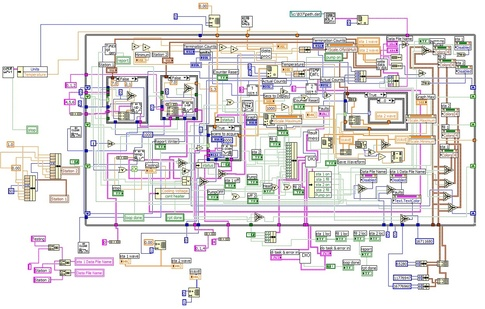
\includegraphics[width=0.9\textwidth]{mess}
    \caption{
        An example of a complex program represented with blocks connected by lines;
        screenshot from \protect\cite{fig_mess}
    }
    \label{fig:mess}
\end{figure}

This problem does not occur in the second most popular VPL representation: the ``snap-together block-based''.

There, the code is presented and manipulated in terms of visual blocks, which can be dragged and dropped by mouse and snapped together like jigsaw puzzle pieces. This representation is self-structuring and designed to resemble the familiar text-based, indent-structured representations.

% advantages and disadvantages of VPLs

\clearpage
\section{Screenshots}\label{sec:screenshots}
This section presents screenshots that show examples of visual programming languages that fall into each of the categories discussed in Section \ref{sec:vpls}.

% This is better, but no source:
%\subsubsection{Design}
%\begin{figure}[h!]
%\centering 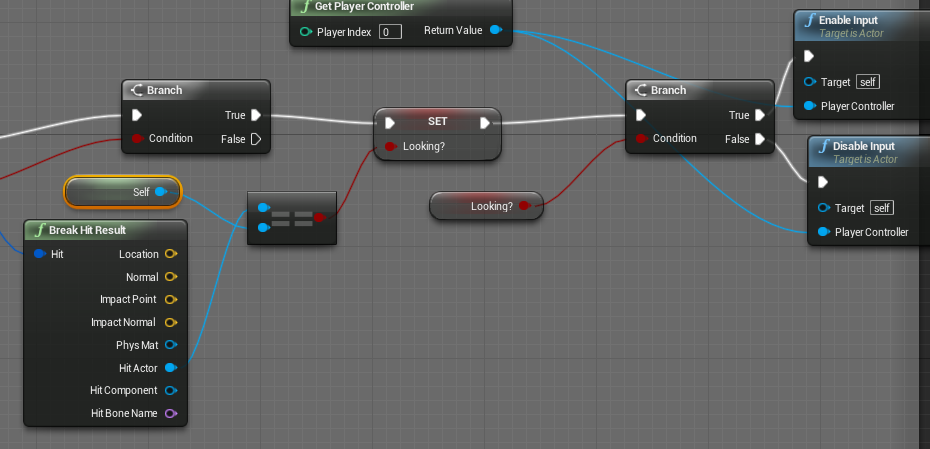
\includegraphics[width=0.9\textwidth]{blueprint_more}
%\caption{}
%\label{fig:blueprint_more}
%\end{figure}

\begin{figure}[h!]
    \centering 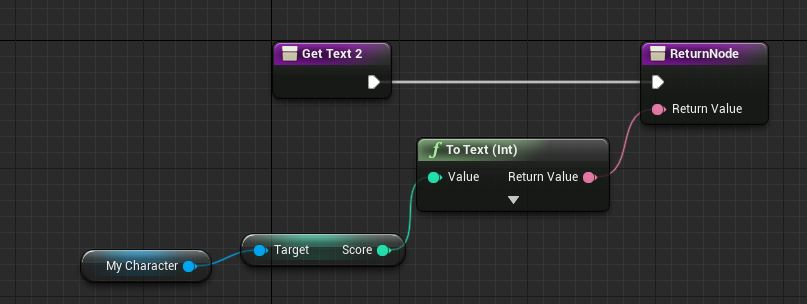
\includegraphics[width=0.9\textwidth]{blueprint}
    \caption{
        Blueprints Visual Scripting system;
        An example of a ``line-connected block-based'' \acrshort{vpl};
        screenshot from \protect\cite{fig_blueprint}
    }
    \label{fig:blueprint}
\end{figure}

\begin{figure}[h!]
    \centering 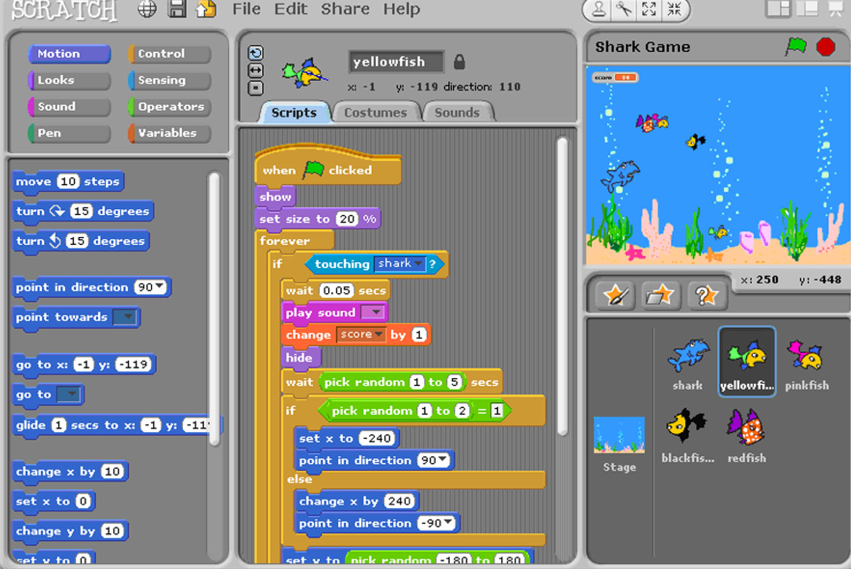
\includegraphics[width=0.9\textwidth]{scratch}
    \caption{
        MIT Scratch programming language editor;
        An example of a ``snap-together block-based'' \acrshort{vpl};
        screenshot from \protect\cite{fig_scratch}
    }
    \label{fig:scratch}
\end{figure}

\begin{figure}[h!]
    \centering 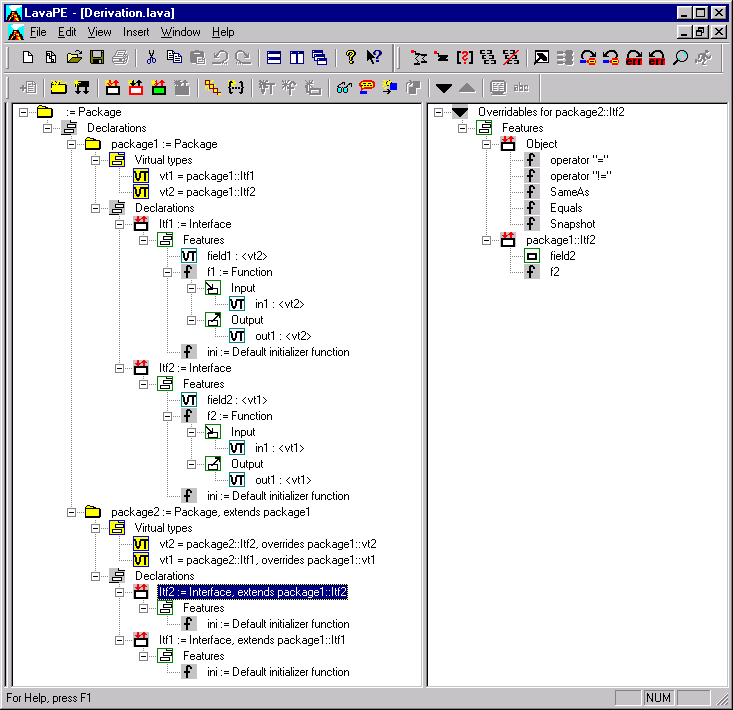
\includegraphics[width=0.75\textwidth]{lava}
    \caption{
        Lava programming language editor;
        An example of a ``list-based'' \acrshort{vpl};
        screenshot from \protect\cite{fig_lava}
    }
    \label{fig:lava}
\end{figure}

\begin{figure}[h!]
    \centering 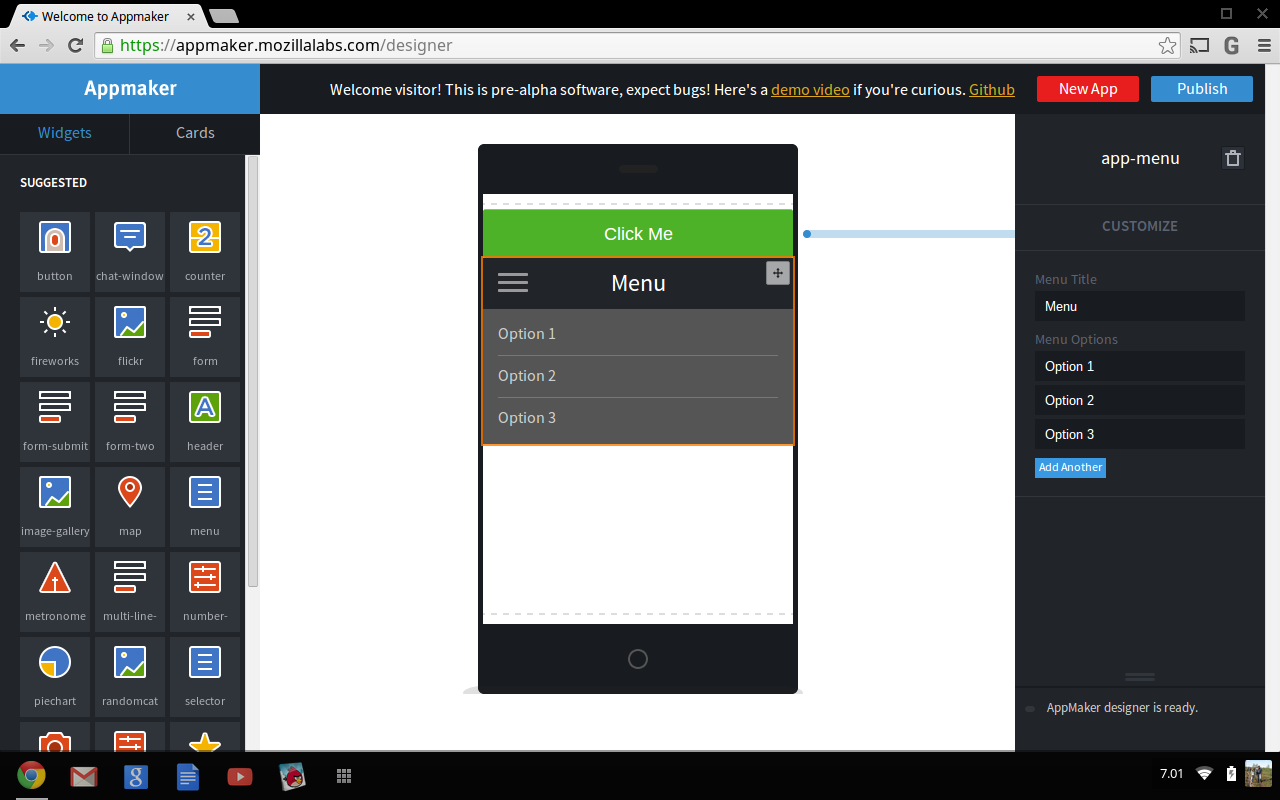
\includegraphics[width=0.9\textwidth]{appmaker}
    \caption{
        Mozilla Appmaker;
        An example of a ``GUI-based'' \acrshort{vpl};
        screenshot from \protect\cite{fig_appmaker}
    }
    \label{fig:appmaker}
\end{figure}

\begin{figure}[h!]
    \centering 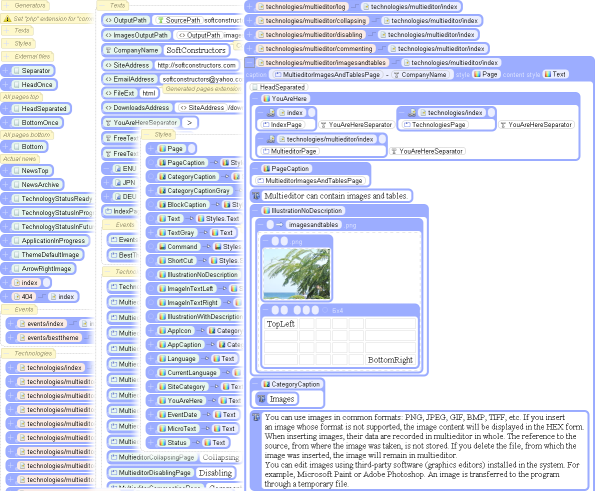
\includegraphics[width=0.9\textwidth]{stroy}
    \caption{
        StroyCode editor;
        An example of a ``nested'' \acrshort{vpl};
        screenshot from \protect\cite{fig_stroy}
    }
    \label{fig:stroy}
\end{figure}

\begin{figure}[h!]
    \centering 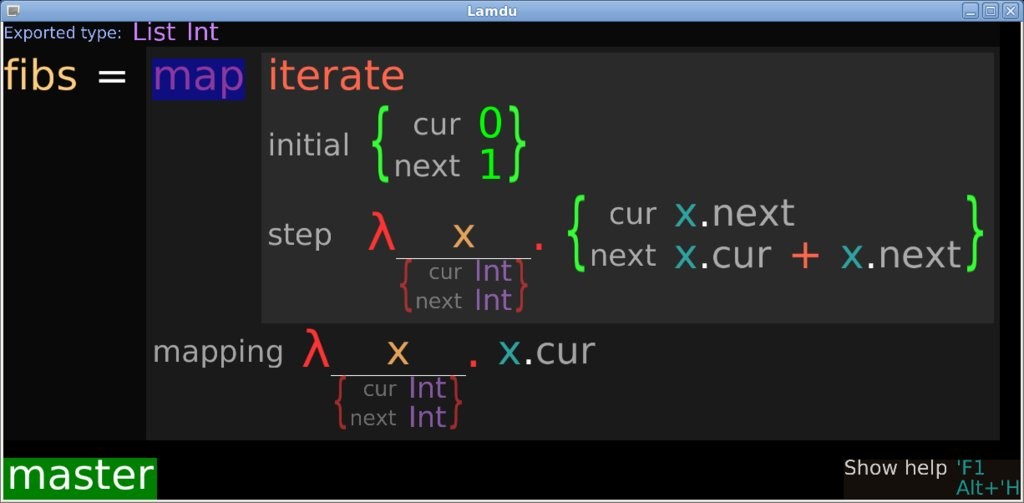
\includegraphics[width=0.9\textwidth]{lamdu}
    \caption{
        Lamdu visual environment;
        An example of an ``enhanced text'' \acrshort{vpl};
        screenshot from \protect\cite{fig_lamdu}
    }
    \label{fig:lamdu}
\end{figure}

\begin{figure}[h!]
    \centering 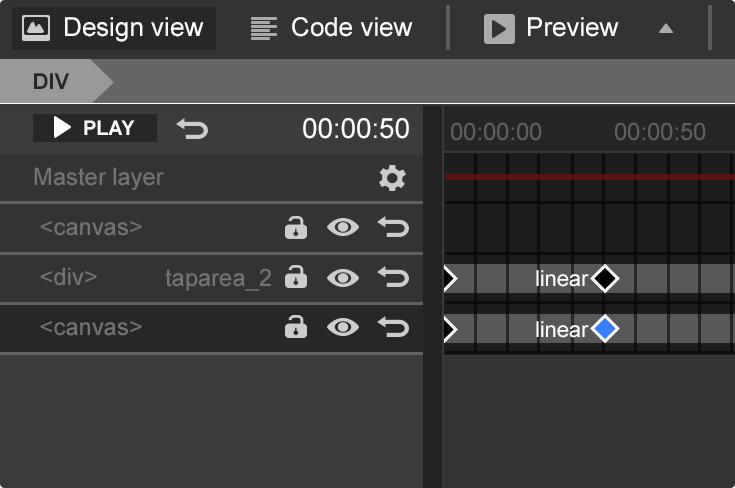
\includegraphics[width=0.75\textwidth]{google_web_designer}
    \caption{
        Google Web Designer;
        An example of a ``timeline-based'' \acrshort{vpl};
        screenshot from \protect\cite{fig_google_web_designer}
    }
    \label{fig:google_web_designer}
\end{figure}

\begin{figure}[h!]
    \centering 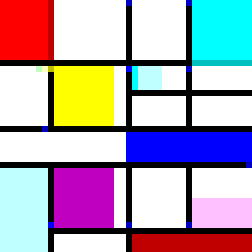
\includegraphics[width=0.5\textwidth]{piet}
    \caption{
        The esoteric programming language Piet;
        An example of an esoteric \acrshort{vpl};
        screenshot from \protect\cite{fig_piet}
    }
    \label{fig:piet}
\end{figure}

\begin{figure}[h!]
    \centering 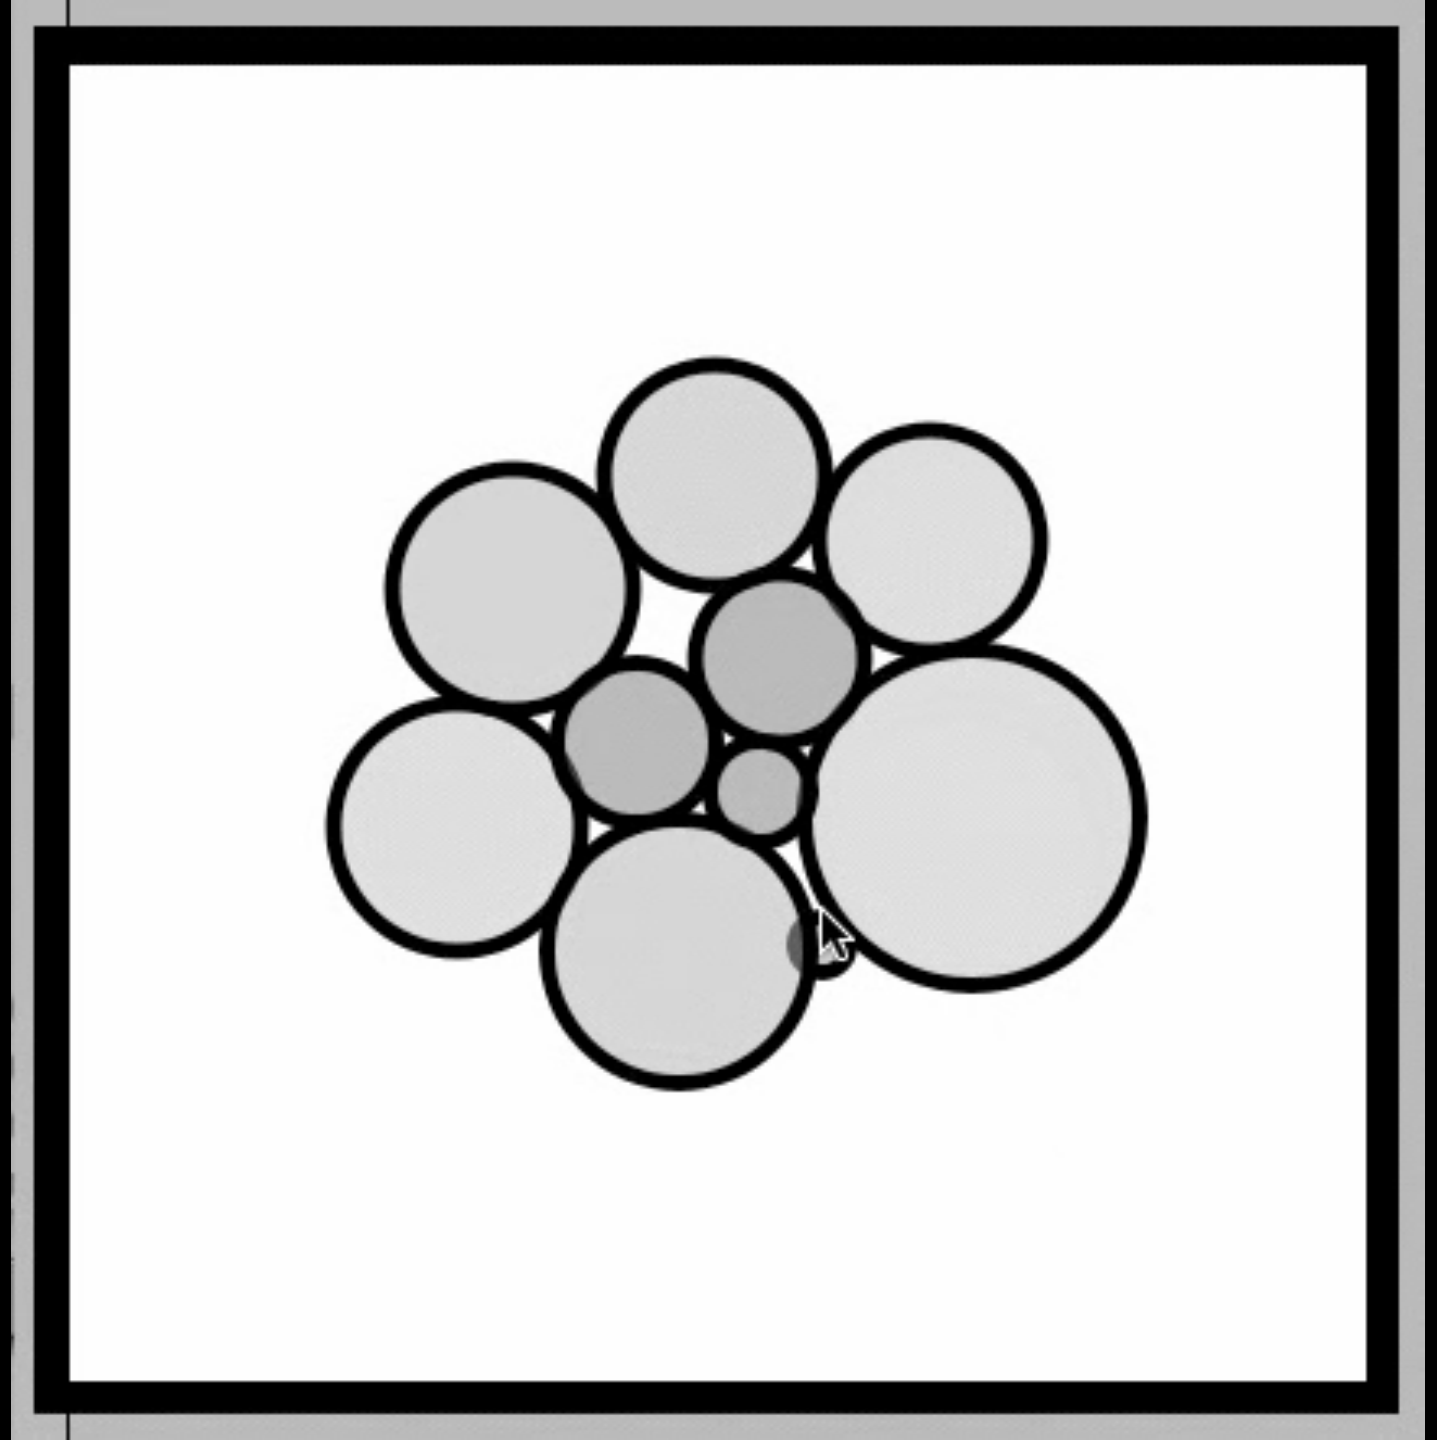
\includegraphics[width=0.5\textwidth]{lily}
    \caption{
        ``Lily was a browser-based, visual programming environment written in JavaScript.''\protect\cite{lily_github};
        An example of an experimental \acrshort{vpl};
        screenshot from \protect\cite{fig_lily}
    }
    \label{fig:lily}
\end{figure}

\begin{figure}[h!]
    \centering 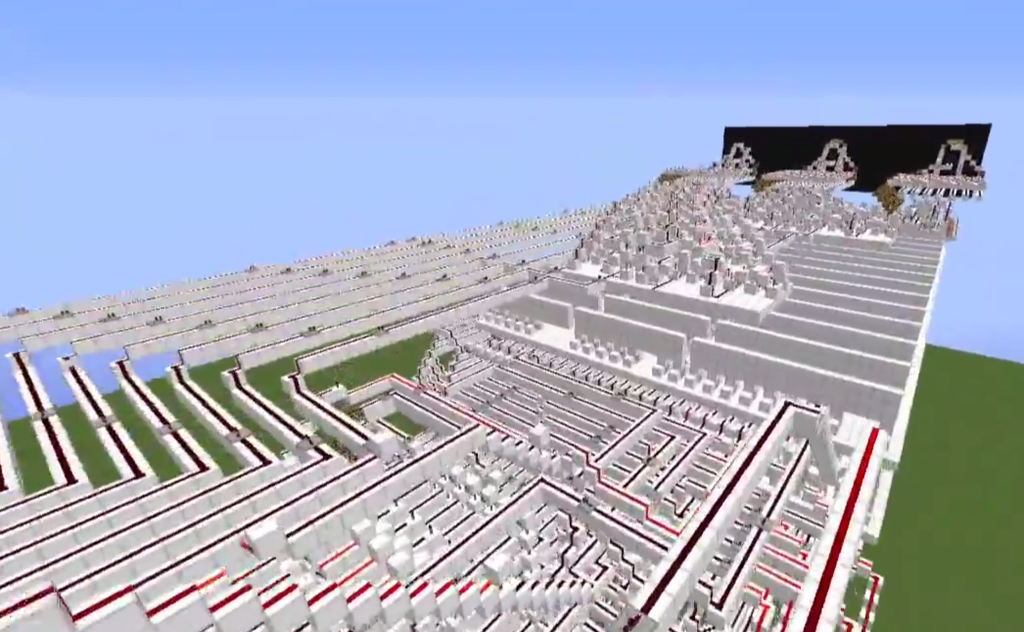
\includegraphics[width=0.9\textwidth]{minecraft}
    \caption{
        Minecraft\cite{minecraft_site} can be considered a visual programming lanugage.
        It's an example of a ``game-based'' \acrshort{vpl};
        ``[S]omeone has created a fully programmable computer using Minecraft''\cite{snapshots};
        screenshot from \protect\cite{fig_minecraft}
    }
    \label{fig:minecraft}
\end{figure}
